%!TeX program = xelatex
%Do not change
\documentclass[12pt, oneside]{article}
\usepackage{amssymb,amsmath}
\usepackage[margin=1in]{geometry}
\usepackage{textpos}
\usepackage{float}
%\usepackage{color}
\usepackage{graphicx}
\usepackage[inter-unit-product =\cdot]{siunitx}
%\usepackage{tikz}
%\usetikzlibrary{positioning}
%\usepackage{tikz-3dplot}
%\usepackage{pgfopts}
%\usepackage{wasysym}
%\usepackage{stanli}

% You may add the packages you need here
\begin{document}

\begin{center}
\textbf{\Large Project 1}

\textbf{Due 19 Feb 2021}
\end{center}

After doing some research into different styles and designs, Dr. Smith has decided to add a leg vise to his woodworking workbench.
He plans to use a ``St. Peter's Cross" mechanism to prevent racking of the vise chop, but he needs to have some analysis done to size the components appropriately.
The critical pieces to size (for this project) are the diameter of the vise screw and the pin connecting the two legs of the cross mechanism.
\begin{itemize}
	\item Assume Dr. Smith applies a force of 20 lbs at the end of the screw handle.
	\item You may choose appropriate dimensions and parameters as needed (for example: handle length and screw pitch). 
	\item \textbf{Hint:} Use simple physics principles (i.e. work done, mechanical advantage) to determine the force in the screw exerted. Formulas that you find via Google will be needlessly complicated (friction effects may be neglected).
	\item Size the screw diameter with a safety factor of 1.7
	\item Size the connector pin with a safety factor of 1.3
\end{itemize}
\begin{figure}[htpb]
	\centering
	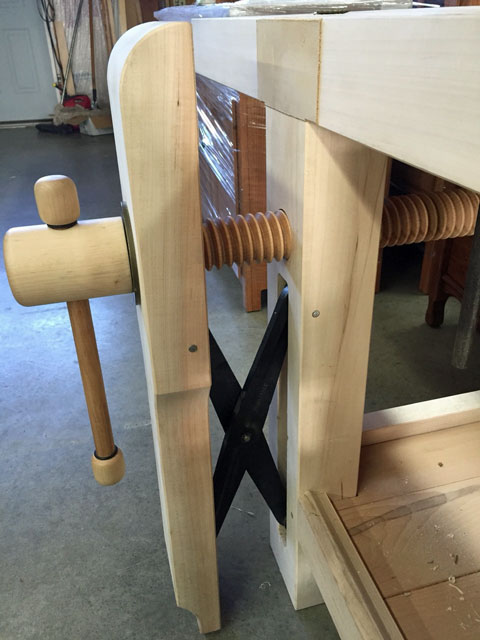
\includegraphics[width=0.4\linewidth]{../../images/stpeterscross}
	\caption{An illustration of a leg vise with a St. Peter's Cross mechanism to prevent racking. This is to serve as an example for the problem, it should not be considered perfectly to scale and you may make assumptions as needed.}
\end{figure}
\end{document}
